\tikzset{every picture/.style={line width=0.75pt}}

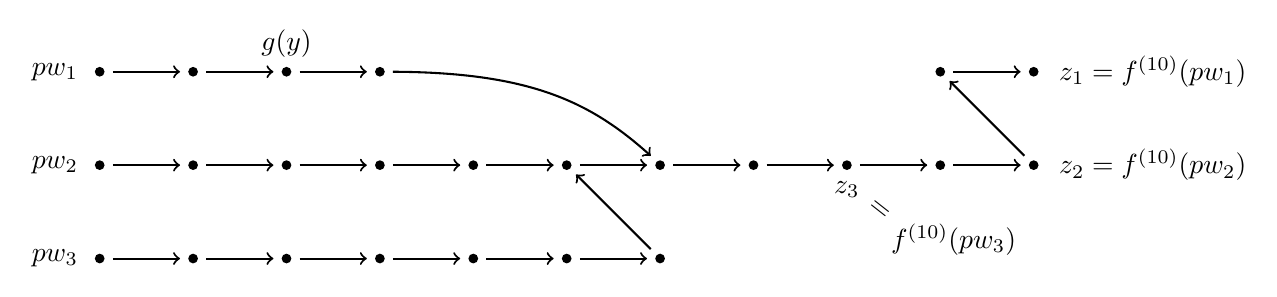
\begin{tikzpicture}[x=0.75pt,y=0.75pt,yscale=-0.9,xscale=0.9]


\draw  [fill={rgb, 255:red, 0; green, 0; blue, 0 }  ,fill opacity=1 ] (38,30) .. controls (38,28.9) and (38.9,28) .. (40,28) .. controls (41.1,28) and (42,28.9) .. (42,30) .. controls (42,31.1) and (41.1,32) .. (40,32) .. controls (38.9,32) and (38,31.1) .. (38,30) -- cycle ;
\draw  [fill={rgb, 255:red, 0; green, 0; blue, 0 }  ,fill opacity=1 ] (88,30) .. controls (88,28.9) and (88.9,28) .. (90,28) .. controls (91.1,28) and (92,28.9) .. (92,30) .. controls (92,31.1) and (91.1,32) .. (90,32) .. controls (88.9,32) and (88,31.1) .. (88,30) -- cycle ;
\draw  [fill={rgb, 255:red, 0; green, 0; blue, 0 }  ,fill opacity=1 ] (138,30) .. controls (138,28.9) and (138.9,28) .. (140,28) .. controls (141.1,28) and (142,28.9) .. (142,30) .. controls (142,31.1) and (141.1,32) .. (140,32) .. controls (138.9,32) and (138,31.1) .. (138,30) -- cycle ;
\draw  [fill={rgb, 255:red, 0; green, 0; blue, 0 }  ,fill opacity=1 ] (188,30) .. controls (188,28.9) and (188.9,28) .. (190,28) .. controls (191.1,28) and (192,28.9) .. (192,30) .. controls (192,31.1) and (191.1,32) .. (190,32) .. controls (188.9,32) and (188,31.1) .. (188,30) -- cycle ;
\draw  [fill={rgb, 255:red, 0; green, 0; blue, 0 }  ,fill opacity=1 ] (38,80) .. controls (38,78.9) and (38.9,78) .. (40,78) .. controls (41.1,78) and (42,78.9) .. (42,80) .. controls (42,81.1) and (41.1,82) .. (40,82) .. controls (38.9,82) and (38,81.1) .. (38,80) -- cycle ;
\draw  [fill={rgb, 255:red, 0; green, 0; blue, 0 }  ,fill opacity=1 ] (88,80) .. controls (88,78.9) and (88.9,78) .. (90,78) .. controls (91.1,78) and (92,78.9) .. (92,80) .. controls (92,81.1) and (91.1,82) .. (90,82) .. controls (88.9,82) and (88,81.1) .. (88,80) -- cycle ;
\draw  [fill={rgb, 255:red, 0; green, 0; blue, 0 }  ,fill opacity=1 ] (138,80) .. controls (138,78.9) and (138.9,78) .. (140,78) .. controls (141.1,78) and (142,78.9) .. (142,80) .. controls (142,81.1) and (141.1,82) .. (140,82) .. controls (138.9,82) and (138,81.1) .. (138,80) -- cycle ;
\draw  [fill={rgb, 255:red, 0; green, 0; blue, 0 }  ,fill opacity=1 ] (188,80) .. controls (188,78.9) and (188.9,78) .. (190,78) .. controls (191.1,78) and (192,78.9) .. (192,80) .. controls (192,81.1) and (191.1,82) .. (190,82) .. controls (188.9,82) and (188,81.1) .. (188,80) -- cycle ;
\draw  [fill={rgb, 255:red, 0; green, 0; blue, 0 }  ,fill opacity=1 ] (38,130) .. controls (38,128.9) and (38.9,128) .. (40,128) .. controls (41.1,128) and (42,128.9) .. (42,130) .. controls (42,131.1) and (41.1,132) .. (40,132) .. controls (38.9,132) and (38,131.1) .. (38,130) -- cycle ;
\draw  [fill={rgb, 255:red, 0; green, 0; blue, 0 }  ,fill opacity=1 ] (88,130) .. controls (88,128.9) and (88.9,128) .. (90,128) .. controls (91.1,128) and (92,128.9) .. (92,130) .. controls (92,131.1) and (91.1,132) .. (90,132) .. controls (88.9,132) and (88,131.1) .. (88,130) -- cycle ;
\draw  [fill={rgb, 255:red, 0; green, 0; blue, 0 }  ,fill opacity=1 ] (138,130) .. controls (138,128.9) and (138.9,128) .. (140,128) .. controls (141.1,128) and (142,128.9) .. (142,130) .. controls (142,131.1) and (141.1,132) .. (140,132) .. controls (138.9,132) and (138,131.1) .. (138,130) -- cycle ;
\draw  [fill={rgb, 255:red, 0; green, 0; blue, 0 }  ,fill opacity=1 ] (188,130) .. controls (188,128.9) and (188.9,128) .. (190,128) .. controls (191.1,128) and (192,128.9) .. (192,130) .. controls (192,131.1) and (191.1,132) .. (190,132) .. controls (188.9,132) and (188,131.1) .. (188,130) -- cycle ;
\draw  [fill={rgb, 255:red, 0; green, 0; blue, 0 }  ,fill opacity=1 ] (238,80) .. controls (238,78.9) and (238.9,78) .. (240,78) .. controls (241.1,78) and (242,78.9) .. (242,80) .. controls (242,81.1) and (241.1,82) .. (240,82) .. controls (238.9,82) and (238,81.1) .. (238,80) -- cycle ;
\draw  [fill={rgb, 255:red, 0; green, 0; blue, 0 }  ,fill opacity=1 ] (288,80) .. controls (288,78.9) and (288.9,78) .. (290,78) .. controls (291.1,78) and (292,78.9) .. (292,80) .. controls (292,81.1) and (291.1,82) .. (290,82) .. controls (288.9,82) and (288,81.1) .. (288,80) -- cycle ;
\draw  [fill={rgb, 255:red, 0; green, 0; blue, 0 }  ,fill opacity=1 ] (338,80) .. controls (338,78.9) and (338.9,78) .. (340,78) .. controls (341.1,78) and (342,78.9) .. (342,80) .. controls (342,81.1) and (341.1,82) .. (340,82) .. controls (338.9,82) and (338,81.1) .. (338,80) -- cycle ;
\draw  [fill={rgb, 255:red, 0; green, 0; blue, 0 }  ,fill opacity=1 ] (238,130) .. controls (238,128.9) and (238.9,128) .. (240,128) .. controls (241.1,128) and (242,128.9) .. (242,130) .. controls (242,131.1) and (241.1,132) .. (240,132) .. controls (238.9,132) and (238,131.1) .. (238,130) -- cycle ;
\draw  [fill={rgb, 255:red, 0; green, 0; blue, 0 }  ,fill opacity=1 ] (288,130) .. controls (288,128.9) and (288.9,128) .. (290,128) .. controls (291.1,128) and (292,128.9) .. (292,130) .. controls (292,131.1) and (291.1,132) .. (290,132) .. controls (288.9,132) and (288,131.1) .. (288,130) -- cycle ;
\draw  [fill={rgb, 255:red, 0; green, 0; blue, 0 }  ,fill opacity=1 ] (338,130) .. controls (338,128.9) and (338.9,128) .. (340,128) .. controls (341.1,128) and (342,128.9) .. (342,130) .. controls (342,131.1) and (341.1,132) .. (340,132) .. controls (338.9,132) and (338,131.1) .. (338,130) -- cycle ;
\draw  [fill={rgb, 255:red, 0; green, 0; blue, 0 }  ,fill opacity=1 ] (388,80) .. controls (388,78.9) and (388.9,78) .. (390,78) .. controls (391.1,78) and (392,78.9) .. (392,80) .. controls (392,81.1) and (391.1,82) .. (390,82) .. controls (388.9,82) and (388,81.1) .. (388,80) -- cycle ;
\draw  [fill={rgb, 255:red, 0; green, 0; blue, 0 }  ,fill opacity=1 ] (438,80) .. controls (438,78.9) and (438.9,78) .. (440,78) .. controls (441.1,78) and (442,78.9) .. (442,80) .. controls (442,81.1) and (441.1,82) .. (440,82) .. controls (438.9,82) and (438,81.1) .. (438,80) -- cycle ;
\draw  [fill={rgb, 255:red, 0; green, 0; blue, 0 }  ,fill opacity=1 ] (488,80) .. controls (488,78.9) and (488.9,78) .. (490,78) .. controls (491.1,78) and (492,78.9) .. (492,80) .. controls (492,81.1) and (491.1,82) .. (490,82) .. controls (488.9,82) and (488,81.1) .. (488,80) -- cycle ;
\draw  [fill={rgb, 255:red, 0; green, 0; blue, 0 }  ,fill opacity=1 ] (538,80) .. controls (538,78.9) and (538.9,78) .. (540,78) .. controls (541.1,78) and (542,78.9) .. (542,80) .. controls (542,81.1) and (541.1,82) .. (540,82) .. controls (538.9,82) and (538,81.1) .. (538,80) -- cycle ;
\draw  [fill={rgb, 255:red, 0; green, 0; blue, 0 }  ,fill opacity=1 ] (488,30) .. controls (488,28.9) and (488.9,28) .. (490,28) .. controls (491.1,28) and (492,28.9) .. (492,30) .. controls (492,31.1) and (491.1,32) .. (490,32) .. controls (488.9,32) and (488,31.1) .. (488,30) -- cycle ;
\draw  [fill={rgb, 255:red, 0; green, 0; blue, 0 }  ,fill opacity=1 ] (538,30) .. controls (538,28.9) and (538.9,28) .. (540,28) .. controls (541.1,28) and (542,28.9) .. (542,30) .. controls (542,31.1) and (541.1,32) .. (540,32) .. controls (538.9,32) and (538,31.1) .. (538,30) -- cycle ;


\draw  [->]  (47,30) -- (83,30) ;
\draw  [->]  (97,30) -- (133,30) ;
\draw  [->]  (147,30) -- (183,30) ;
\draw  [->]  (497,30) -- (533,30) ;

\draw  [->]  (47,80) -- (83,80) ;
\draw  [->]  (97,80) -- (133,80) ;
\draw  [->]  (147,80) -- (183,80) ;
\draw  [->]  (197,80) -- (233,80) ;
\draw  [->]  (247,80) -- (283,80) ;
\draw  [->]  (297,80) -- (333,80) ;
\draw  [->]  (347,80) -- (383,80) ;
\draw  [->]  (397,80) -- (433,80) ;
\draw  [->]  (447,80) -- (483,80) ;
\draw  [->]  (497,80) -- (533,80) ;

\draw  [->]  (47,130) -- (83,130) ;
\draw  [->]  (97,130) -- (133,130) ;
\draw  [->]  (147,130) -- (183,130) ;
\draw  [->]  (197,130) -- (233,130) ;
\draw  [->]  (247,130) -- (283,130) ;
\draw  [->]  (297,130) -- (333,130) ;

\draw  [->]  (335,125) -- (295,85) ;
\draw  [->]  (535,75) -- (495,35) ;

\draw  [->]  (197,30) .. controls (270.33,30.33) and (302.67,46) .. (335,75) ;

\draw (2,30) node [anchor=west] [inner sep=0.75pt]    {$pw_{1}$};
\draw (2,80) node [anchor=west] [inner sep=0.75pt]    {$pw_{2}$};
\draw (2,130) node [anchor=west] [inner sep=0.75pt]    {$pw_{3}$};
\draw (140,24) node [anchor=south] [inner sep=0.75pt]    {$g( y)$};
\draw (440,87) node [anchor=north] [inner sep=0.75pt]    {$z_{3}$};
\draw (552,30) node [anchor=west] [inner sep=0.75pt]    {$z_{1} =f^{( 10)}( pw_{1})$};
\draw (552,80) node [anchor=west] [inner sep=0.75pt]    {$z_{2} =f^{( 10)}( pw_{2})$};
\draw (462,120) node [anchor=west] [inner sep=0.75pt]    {$f^{( 10)}( pw_{3})$};
\draw (454,96) node [anchor=north west][inner sep=0.75pt]  [rotate=-38.18]  {$=$};


\end{tikzpicture}